\documentclass{beamer}
\usetheme{Madrid}

\usepackage{graphicx}
\usepackage{adjustbox}
\usepackage{tikz}
\usepackage{listings}

\usetikzlibrary{automata,arrows}
\pgfmathtruncatemacro\distance{1}

\lstset{language=erlang, basicstyle=\sffamily\footnotesize,
  keywordstyle=\color{blue}, numberstyle=\tiny, numbers=none,
  showspaces=false, showstringspaces=false, frame=tL,
  backgroundcolor=\color{black!5}, morekeywords={send, to, from} }

\title{Extracting Choreography Automata \\ for Program Understanding}
\author{Gabriele Genovese \\ Supervisor: Prof. Cinzia Di Giusto}
\date{\today}

\begin{document}

\frame{\titlepage}

% aim
%

% \begin{frame}{Overview}
% \tableofcontents
% \end{frame}

% This project focuses on the development of distributed systems, particularly on  
% how to assist developers in designing and debugging communication protocols.  
% A distributed system consists of multiple participants collaborating toward a  
% common goal. These participants communicate over a channel, which is often  
% asynchronous.  
% Application development in this context typically relies on programming  
% languages that adopt the actor model. This model is either natively  
% supported or integrated through libraries and frameworks in modern languages.  
% Erlang stands out as the most established language for this paradigm.  
% Developers usually write functions that interact with each other, an approach  
% that contrasts with the academic perspective, where a global specification  
% is first defined, and individual functions are derived from it.  
% This project aims to analyze an existing codebase and extract the global  
% specification from the local specifications. This helps programmers  
% better understand their programs and facilitates debugging.
\section{Introduction}
\begin{frame}{Introduction}
\begin{itemize}
    \item Aim: explore formal model for development of 
    distributed application for protocol specification
\end{itemize}
\bigskip
\begin{center}
\includegraphics[width=0.8\textwidth]{images/crop.png}
\end{center}
\end{frame}

\begin{frame}{Context}
\begin{itemize}
    \item Distributed system: set of \textbf{participants} working for a  
    common goal
    \bigskip
    \item \textbf{Asynchronous} communication channel
    \bigskip
    \item Programming with the \textit{actor model} (Erlang)
    \bigskip
    \item \textit{Send} and \textit{receive} main operations
    \bigskip
    \item Protocols usually designed with \textit{top-down approach} 
\end{itemize}
    
\end{frame}

\begin{frame}{Brief introduction to Choreography Automata}

\begin{itemize}
    \item Choreography: a formal model for distributed systems used
    for protocol specification
    \bigskip
    \item \textbf{Global view}: communication system seen from above
    \bigskip
    \item \textbf{Local view}: point of view of a single participant
    \bigskip
    \item Choreography Automata: a \textit{graphical} way of expressing Choreography
\end{itemize}
\end{frame}

\begin{frame}{Motivations}
\begin{itemize}
    \item \textit{Debugging}, \textit{verification} of 
    concurrent properties (\textit{deadlock}, \textit{liveness}, etc...), 
    \textit{program understanding}
    \bigskip
    \item Bottom-up approach like the one used in programming
    \bigskip
    \item Chorer: a prototype for a static analyzer that extract Choreography Automata
\end{itemize}
\end{frame}


\begin{frame}{Case study: Dining philosopher}
\begin{itemize}
    \item ! : send
    \item ? : receive
\end{itemize}
    \begin{figure}[ht]
    \centering
    % \makebox[\textwidth][c]{
    \resizebox{0.7\textwidth}{!}{%
    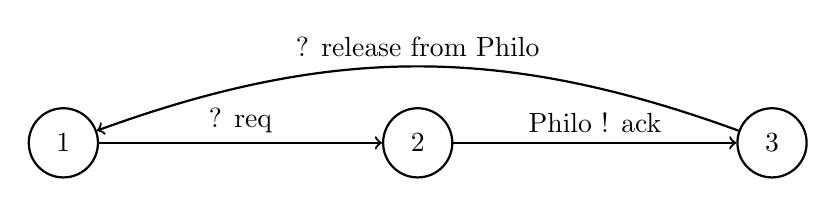
\begin{tikzpicture}[node distance={45mm}, thick, main/.style = {draw, circle}] 
        \node[state] (n_1) {1};
        \node[state] (n_2) [right of=n_1] {2};
        \node[state] (n_3) [right of=n_2] {3};
        
        \draw[->] (n_1) -- node[midway, above, pos=0.5] {? req} (n_2);
        \draw[->] (n_2) -- node[midway, above, pos=0.5] {Philo ! ack} (n_3);
        \draw[->] (n_3) to [out=160,in=20] node[midway, above, pos=0.5] {? release from Philo} (n_1);
    \end{tikzpicture}
    }
    % }%
    \caption{Local view of a fork.}
    \label{graph:forklocal}
    \end{figure}
    \begin{figure}[ht]
    \centering
    % \makebox[\textwidth][c]{
    \resizebox{0.9\textwidth}{!}{%
        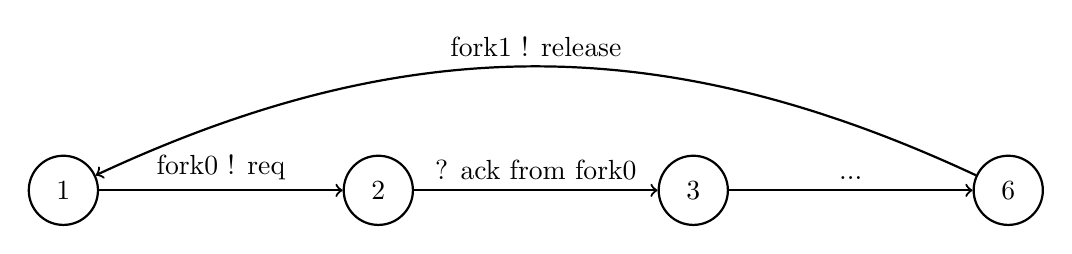
\begin{tikzpicture}[node distance={40mm}, thick, main/.style = {draw, circle}] 
            \node[state] (n_1) {1};
            \node[state] (n_2) [right of=n_1] {2};
            \node[state] (n_3) [right of=n_2] {3};
            \node[state] (n_4) [right of=n_3] {6};
            
            \draw[->] (n_1) -- node[midway, above, pos=0.5] {fork0 ! req} (n_2);
            \draw[->] (n_2) -- node[midway, above, pos=0.5] {? ack from fork0} (n_3);
            \draw[->] (n_3) -- node[midway, above, pos=0.5] {...} (n_4);
            \draw[->] (n_4) to [out=155,in=25]  node[midway, above, pos=0.5] {fork1 ! release} (n_1);
        \end{tikzpicture}
        }
    % }%
    \caption{Local view of a philosopher.}
    \label{graph:philolocal}
    \end{figure}
\end{frame}

\begin{frame}{Global view example}

\begin{figure}[t]
\centering
% \makebox[\textwidth][c]{
\resizebox{\textwidth}{!}{%
    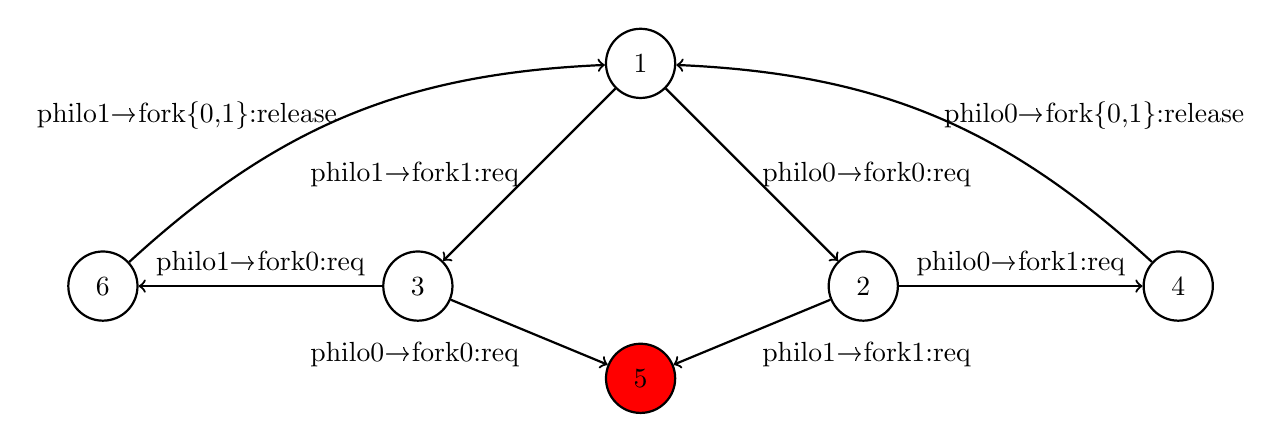
\begin{tikzpicture}[node distance={40mm}, thick, main/.style = {draw, circle}] 
        \node[state] (n_1) {1};
        \node[state] (n_2) [below right of=n_1] {2};
        \node[state] (n_3) [below left of=n_1] {3};
        \node[state] (n_4) [right of=n_2] {4};
        \node[state] (n_5) [below of=n_1, fill=red] {5};
        \node[state] (n_6) [left of=n_3] {6};
        
        \draw[->] (n_1) -- node[midway, right, pos=0.5] {philo0→fork0:req} (n_2);
        \draw[->] (n_1) -- node[midway, left, pos=0.5] {philo1→fork1:req} (n_3);
        \draw[->] (n_2) -- node[midway, below right, pos=0.5] {philo1→fork1:req} (n_5);
        \draw[->] (n_3) -- node[midway, below left, pos=0.5] {philo0→fork0:req} (n_5);
        \draw[->] (n_2) -- node[midway, above, pos=0.5] {philo0→fork1:req} (n_4);
        \draw[->] (n_4) to[bend right=20] node[midway, right, pos=0.5] {philo0→fork\{0,1\}:release} (n_1);
        \draw[->] (n_3) -- node[midway, above, pos=0.5] {philo1→fork0:req} (n_6);
        \draw[->] (n_6) to[bend left=20] node[midway, left, pos=0.5] {philo1→fork\{0,1\}:release} (n_1);
    \end{tikzpicture}
    }
% }%
\caption{Global view of the dining philosophers example.}
\label{graph:philoglobal}
\end{figure}
\end{frame}


\begin{frame}{Characteristics of the tool}
\begin{itemize}
    \item Automatic \textbf{bottom-up} extraction
    \bigskip
    \item \textbf{Over-approximated} approach when computing the globalview
    \bigskip
    \item Always capture the good behaviors, and highlight possible misbehavior
    \bigskip
    \item Applicable to mainstream languages
\end{itemize}
\end{frame}

\section{Chorer}
\begin{frame}{Chorer}
Proof of Concept for a static analyzer
developed as part of my Bachelor’s thesis at the University of Bologna.
Old state:
\bigskip
\begin{itemize}
    \item Few working examples and no case study
    \bigskip
    \item Some important feature missing (basic use of functions)
    \bigskip
    \item Very difficult to use and understand
\end{itemize}
\end{frame}

\section{Contributions}
\begin{frame}{Contributions}
\begin{itemize}
    \item Formalization journey began (attributed grammar)
    \bigskip
    \item Lots of improvements on the codebase (feature, bug, misc)
    \bigskip
    \item Benchmarks suite improved and case studies created 
\end{itemize}
\end{frame}

\begin{frame}{Attributed grammar}
\begin{itemize}
    \item Aim: generalize some aspect of the tool
    \bigskip
    \item Formal grammar enriched with attributes assigned to symbols 
    that define how these attributes are computed.
    \bigskip
    \item Used in compilers and parsers design
    \bigskip
    \item Begin a formalization and refactoring process for localviews. 
\end{itemize}
\end{frame}


% parlare del bottom up e degli attributi
\begin{frame}[fragile]{Attributes}
Bottom-up technique. Attributes found:
\bigskip
\begin{itemize}
    \item Nodes and Edges with Labels: used to show the automata
    \bigskip
    \item First and Last Node of the automata: used to link some production 
    \bigskip
    \item Context and Returned Variable: used to manage process identifiers and data in general
\end{itemize}
\end{frame}

% Thanks to the attributed grammar, new feature where developed

\begin{frame}{Improvements}
Feature:
\begin{itemize}
    \item Value passing in functions (localview)
    \bigskip
    \item ANY data overapproximation added (globalview)
    \bigskip
    \item Improvements on CLI argument parsing, error and warning report
    \bigskip
    \item Benchmark suite and testing enhanced 
    \bigskip
    \item Some important bugs fixed
\end{itemize}
\end{frame}

\begin{frame}{Benchmarks - Empirical data}
\begin{itemize}
    \item Examples made by myself
    \item Show some empirical data about the output produced
    \item Algorithm $O(n!)$ but in practice very efficient 
\end{itemize}

\begin{table}[!ht]
\centering
\begin{tabular}{|c|c|c|c|c|c|c|c|}
\hline
Example & Tot LV & GV Nodes & GV Edges & Warns & Errors & Time \\ 
\hline
async & 3 & 7 & 6 & 0 & 0 & 0.194s \\ 
dining & 3 & 45 & 72 & 0 & 2 & 0.232s \\ 
account & 3 & 28 & 39 & 0 & 2 & 0.211s \\ 
if-cases & 4 & 148 & 210 & \textbf{185} & 30 & 0.525s \\ 
foo6 & 5 & 9 & 9 & 15 & 2 & 0.190s \\ 
foo7 & 3 & 149 & 229 & 0 & 6 & 0.513s \\ 
foo8 & 5 & \textbf{561} & \textbf{560} & 0 & \textbf{191} & \textbf{3.590s} \\ 
\hline
\end{tabular}
\caption{Global view empirical data}
\label{tab:gvbench}
\end{table}
\end{frame}

% dire più informazioni su stati, warning e errori

\begin{frame}{Benchmarks - Correctness}
Set ground for a precision benchmark (a correct version of the 
global view must be present):
\begin{itemize}
    \item True: the global view given in output is the same of its
    correct version
    \item False: there are some difference
\end{itemize}

\begin{table}[!ht]
\centering
\begin{tabular}{|c|c|}
\hline
Example & Check \\ 
\hline
unknown & False \\ 
async & True \\ 
ticktackloop & True \\ 
ticktackstop & False \\ 
customer & False \\ 
\hline
\end{tabular}
\caption{Global view correctness data}
\label{tab:corrbench}
\end{table}
\end{frame}

\section{Conclusion}
\begin{frame}{Conclusion}
Key contributions:
\bigskip
\begin{itemize}
    \item Study of the requirements and of the challenges
    \bigskip
    \item Several improvements to the codebase and test suite
    \bigskip
    \item Set groundwork for a formalization process and refactoring
\end{itemize}

\end{frame}


\begin{frame}{Future works}
\begin{itemize}
    \item Continue the formalization and refactoring process
    \bigskip
    \item Extend correctness benchmarks
    \bigskip
    \item Continue feature (new keyword or BIF) and bug fix process
\end{itemize}
\end{frame}


\begin{frame}{}
\centering
Thank you for your attention!
\end{frame}


\end{document}